\chapter{Simulation tools and Introduction to Baadal Architecture}

Getting started with theory of Software defined networking, we tested our grasp on literature by performing simulations with basic topologies and scripts. 

For basic experimentation, we started with the mininet for creating customised topologies using python scripts. Later on we created the baadal architecture using physical host (baadal sandbox).
We will also discuss the baadal networking architecture as a prerequisite to move forward with the installation of baadal sandbox and further development.

\section{Mininet}

Mininet is a network emulator. It creates a network of virtual hosts, switches, controllers, and links. It runs standard Linux network software and supports OpenFlow for flexible custom routing and software defined networking. Some of the features of mininet are: 
\begin{itemize}
    \item A simple and inexpensive \textbf{network testbed} provision for developing OpenFlow applications
    \item enables complex topology testing, without the need to wire up a physical network
    \item enables multiple concurrent developers to work independently on the same topology
    \item provides an extensible Python API for network creation and experimentation
\end{itemize}

\section{Overview of Baadal Networking Architecture}
In this section we will present the overview of the baadal networking architecture. The components comprising the architecture are mentioned below:-

\begin{itemize}
    \item \textbf{NAT} Network Address tanslator is the component which act as firewall for the baadal network. All the traffic of the baadal network pass through it. Internal baadal nodes communicate to the internet via this interface only. It is implemented on an OpenVswitch which is hosted in a physical machine with Ubuntu as its OS.
    \item \textbf{Hardware Switch} It is a physical switch which is connected to all the other networking components including the physical hosts, Baadal Controller, Filer and NAT.
    \begin{figure}[h]
\caption{Overview of Baadal Architecture}
\centering
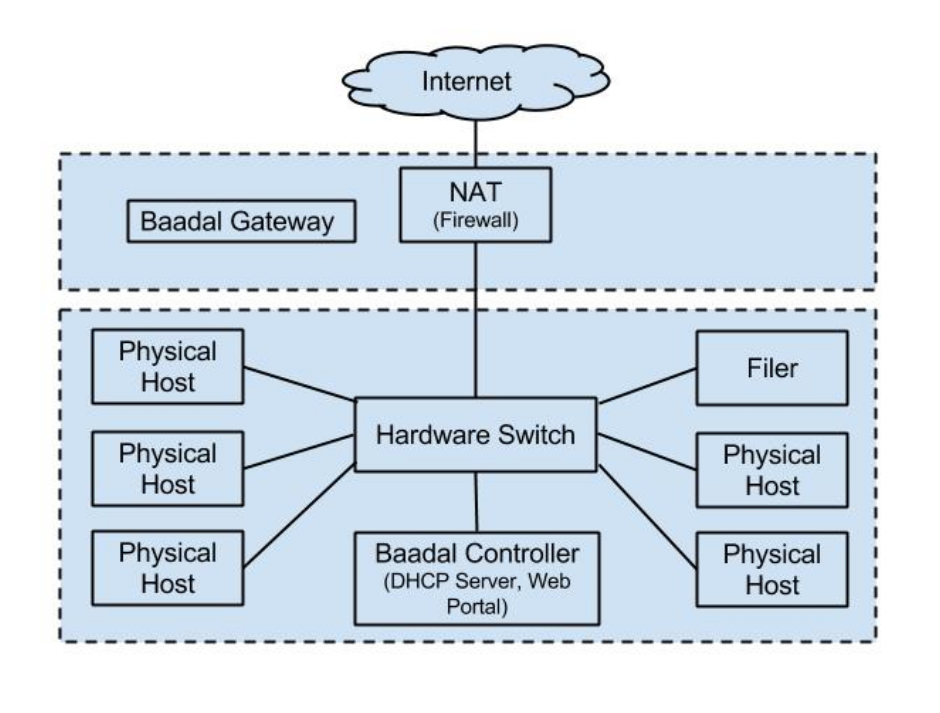
\includegraphics[width=0.9\textwidth]{Baadal_architecture}
\end{figure}
    \item \textbf{Baadal Controller} This component is responsible for providing web portal where a user can request a VM, a facutly supervisor approves it and an administrator can commission it. The main function of it is to be central controlling element alongwith hosting components like DHCP server, TFTP server, scheduler etc.
    
    \item \textbf{Filer} For all the physical hosts Filer is the network file manager. On request of virtual machines, controller hosts the virtual hard disk. But additional hard disk is allocated in the filer machine.
    
    \item \textbf{Physical host} These are responsible for hosting all the VMs created by the user. KVM is the hypervisor layer in the physical host.
    
\begin{figure}[h]
\caption{Physical host architecture}
\centering
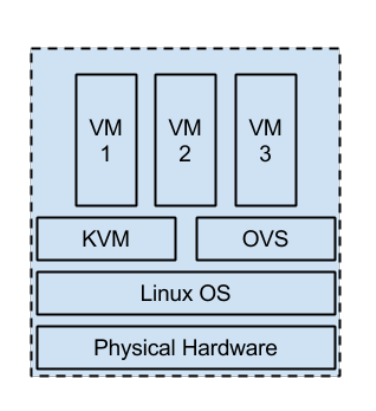
\includegraphics[width=0.5\textwidth]{PhysicalHost_architecture}
\end{figure}
\end{itemize}

%\section{Implementation of Virtual Network using OpenDaylight}